% !TEX encoding = UTF-8 Unicode
\documentclass[a4paper,12pt]{article}
\usepackage{graphicx}
\usepackage{CJK}

\begin{CJK}{UTF8}{gbsn}

	\title{个人简历}
	\author{罗晓俊}

\end{CJK}

\begin{document}
	\begin{CJK}{UTF8}{gbsn}

		\maketitle{}

		% 照片
		\begin{figure}[h]
			\centering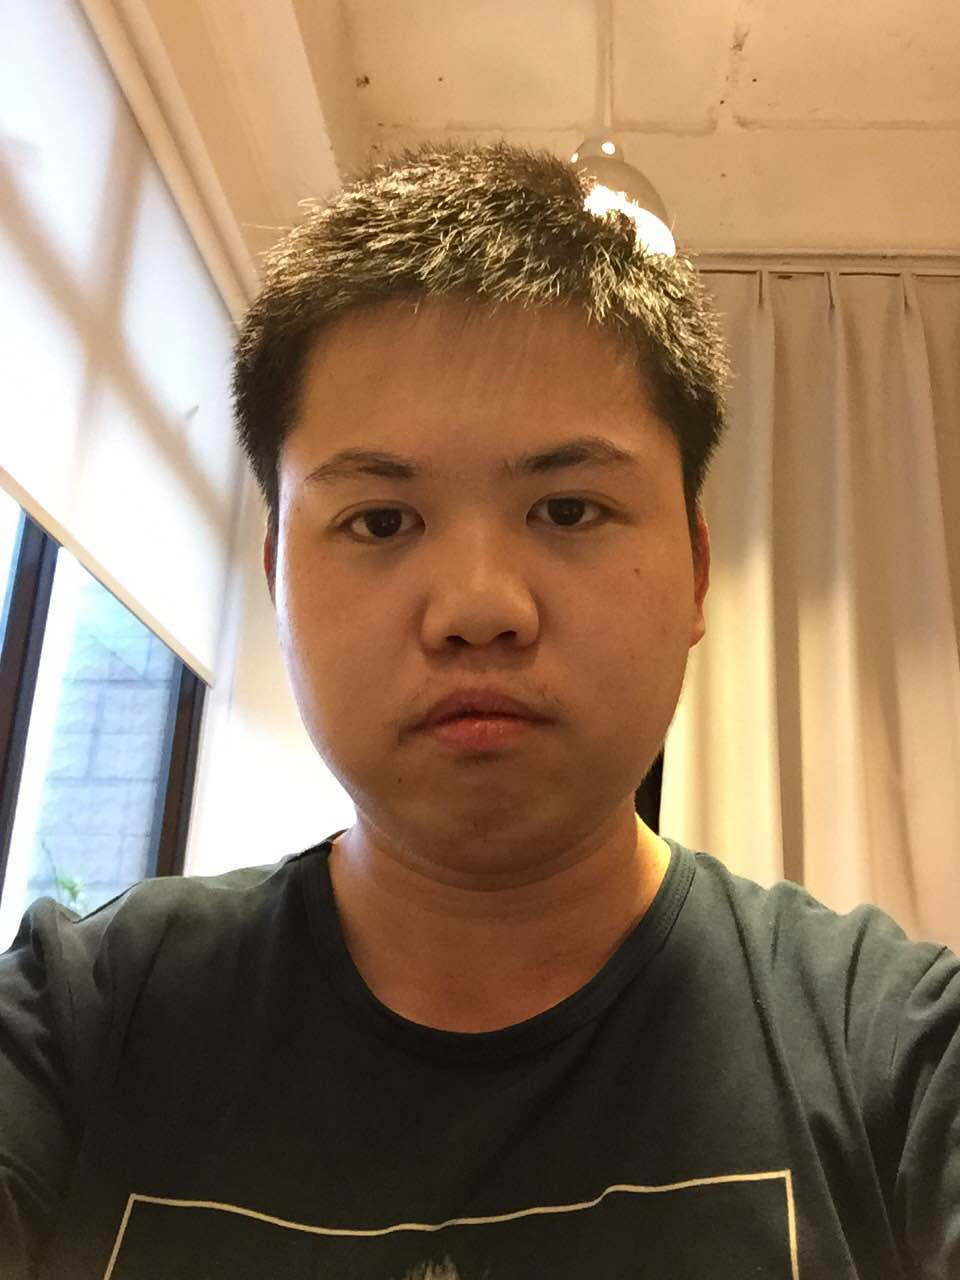
\includegraphics[height=100px]{webwxgetmsgimg.jpeg}
		\end{figure}

		% 联系方式
		\section{联系方式}
			\begin{itemize}
				\item{邮箱: luoxiaojun1992@sina.cn}
				\item{手机: 18616255973}
			\end{itemize}

		% 个人简介
		\section{个人简介}
			\begin{itemize}
				\item{崇尚极客精神,崇尚开源,喜欢学习和钻研技术。未来的目标是成为一名架构师。}
				\item{希望加入一家业务稳定、有技术追求、有创新精神的团队。}
				\item{爱好摄影、桌球、军事、航空。}
			\end{itemize}
		
		% 教育经历
		\section{教育经历}
			\begin{itemize}
				\item{南昌工程学院 电气工程及其自动化 全日制本科 2014年毕业}
			\end{itemize}
		
		% 工作经历
		\section{工作经历}
			\begin{itemize}
				\item{2014.1 - 2015.10 融锋网络科技(上海)有限公司}
				\item{2015.11 - 2016.7 上海雀夸网络科技有限公司}
				\item{2016.7 - 2016.12 上海安个家信息技术有限公司}
				\item{2017.1 - 至今 上海乾升乾金融信息服务有限公司}
			\end{itemize}
		
		% 专业技能
		\section{专业技能}
			\begin{itemize}
				\item{掌握PHP语言}
				\item{掌握Linux、Mac开发环境}
				\item{掌握MySQL使用}
				\item{掌握Redis使用}
				\item{掌握Git、SVN版本控制}
				\item{掌握Markdown文档编写}
				\item{熟悉jQuery}
				\item{熟悉Yii、Laravel、ThinkPHP框架}
				\item{熟悉框架基本原理}
				\item{熟悉PSR-2编码规范}
				\item{熟悉LNMP环境搭建}
				\item{熟悉单元测试、PHPUnit、Mockery}
				\item{了解HTTP、HTTP2、TCP/IP协议}
				\item{了解RESTful,避免分布式事务实现方案}
				\item{了解Redis协议、持久化方式}
				\item{了解MySQL原理,事务、索引、联接、分区等}
				\item{了解PHP内核原理}
				\item{了解Nginx模块开发}
				\item{了解常用的消息队列,如ActiveMQ、Kafka、NSQ、RabbitMQ}
				\item{了解常用设计模式}
				\item{了解JSX、Virtual DOM原理}
				\item{了解Go语言,有一些开发经验}
				\item{了解Angular,用cordova\&ionic开发过淘宝客APP}
				\item{了解thrift,公司项目使用过,框架中集成过}
				\item{了解protobuf、gRPC}
				\item{了解服务化相关知识}
				\item{了解常用排序、查找算法、树的深度广度优先遍历、树的翻转}
			\end{itemize}
		
		% 项目经验
		\section{项目经验(上海乾升乾金融信息服务有限公司)}
			\begin{itemize}
				\item{代码重构优化}
				\item{灰度发布和测试方案}
                			\item{PHP7.0升级}
                			\item{提出技术设计评审、代码评审方案} 
				\item{百度金融、腾讯广点通API对接}
				\item{分期贷模块}
				\item{贷上钱借贷APP迭代工作,负责分配任务、项目估时、接口开发、上线}
				\item{短信基础服务,新增短信渠道对接}
			\end{itemize}
			
		\section{项目经验(上海安个家信息技术有限公司)}
			\begin{itemize}
				\item{监控报警系统二次开发}
				\item{房源APP积分模块重构}
				\item{电话基础服务重构}
				\item{链接小区数据爬虫防封禁策略}
				\item{对接预拨号基础服务}
				\item{房源APP迭代接口开发}
			\end{itemize}
		
		\section{项目经验(上海雀夸网络科技有限公司)}
			\begin{itemize}
				\item{返利商城维护、迭代}
				\item{OA系统迭代}
				\item{商城论坛维护}
			\end{itemize}
			
		\section{项目经验(融锋网络科技(上海)有限公司)}
			\begin{itemize}
				\item{电商外包开发}
				\item{微信公众号管理平台开发}
			\end{itemize}
		
		% 开源贡献
		\section{开源贡献}
		 	\begin{itemize}
				\item{GitHub: https://github.com/luoxiaojun1992}
				\item{PHP框架: https://github.com/luoxiaojun1992/lb\_framework.git}
				\item{Yii2-Queue优化: https://github.com/luoxiaojun1992/yii2-queue}
				\item{Redis连接池: https://github.com/luoxiaojun1992/redis-proxy}
				\item{Nginx灰度模块: https://github.com/luoxiaojun1992/nginx\_http\_gray\_module}
				\item{Telegraf插件: https://github.com/luoxiaojun1992/telegraf}
				\item{WebAssembly学习: https://github.com/luoxiaojun1992/webassembly-learning}
			\end{itemize}
		
		% 个人博客
		\section{个人博客}
			\begin{itemize}
				\item{https://my.oschina.net/luoxiaojun1992/blog}
			\end{itemize}

	\end{CJK}
\end{document}
